
\chapter{Algorithm Design Limitations}\label{ch:design} 
% purpose of this chapter and what it brings
This chapter analyzes the implied limitations by the data generated and the used algorithmic methods in literature for geometry feature extraction.  These limitations will be used to from a new algorithm based upon methods solving the issues at hand. 

% how the chapter is build up
First the goal of the new proposed algorithm is set. Next, the limitations of the data output from the vision system as described in Chapter \ref{ch:hardware} are discussed. Followed by a literature review on the previous work done on feature extraction based on laser vision with a discussion on the limitations of the used methods. 

\section{Objective}
% the goal of the algorithm
\textbf{The goal of the image processing algorithm is to detect deposition feature height and width.} The experimental hardware setup used for design of this algorithm is as follows where results from Chapter \ref{ch:hardware} are used. 

% hardware conditions used to test and achieve the goal
\begin{itemize}
\item \textbf{Reverse Configuration} This triangulation configuration is used for analysis and development of the algorithm. 
\item \textbf{Reflective Material} To make it possible to detect difference between the depostion and the bed a reflective white silicon based material is used as deposition.
\item \textbf{Low-Quality Hardware} To test for robustness against suboptimal conditions low-quality hardware as in the camera and line-laser are used.
\end{itemize}

% focus of the algorithm
\skippar
The follwing subgoals are set for the algorithm design which are focused towards the application of real-time control of the deposition geometry.
\begin{itemize}
\item \textbf{Fast Mathematical Operations} With real-time control purposes in mind the focus is to use simple mathematical image processing methods to allow for high frame rates. 
\item \textbf{Deterministic Behavior} To keep the amount of jitter acceptable, iterative mathematical operations should be avoided.
\item \textbf{Robustness} The algorithm should be robust against noise and changing conditions. 
\item \textbf{Flexibility} The influence of different image signatures due to the use of other hardware should be minimized as much as possible. 
\item \textbf{Automated} It should be avoided to use algorithms which demand settings. Hardcoded constants should be avoided as much as possible. 
\end{itemize}

\section{Data limitations} \label{sc: data limitations}
% explain need for data analysis of images
To achieve robustness against the suboptimal conditions the data generated by the camera is analyzed to identify the effect of the low-quality components on the images created. A typical image from the camera is shown in Figure \ref{fig: data_problem} where the laser is positioned at the bottom of the image. The image shows little similarity with the predicted output as in Figure \ref{fig:profile}. The line is supposed to accurately follow the geometry of the deposition such that it can be used to measure width and height.
\begin{figure}[!h]
	\centering
	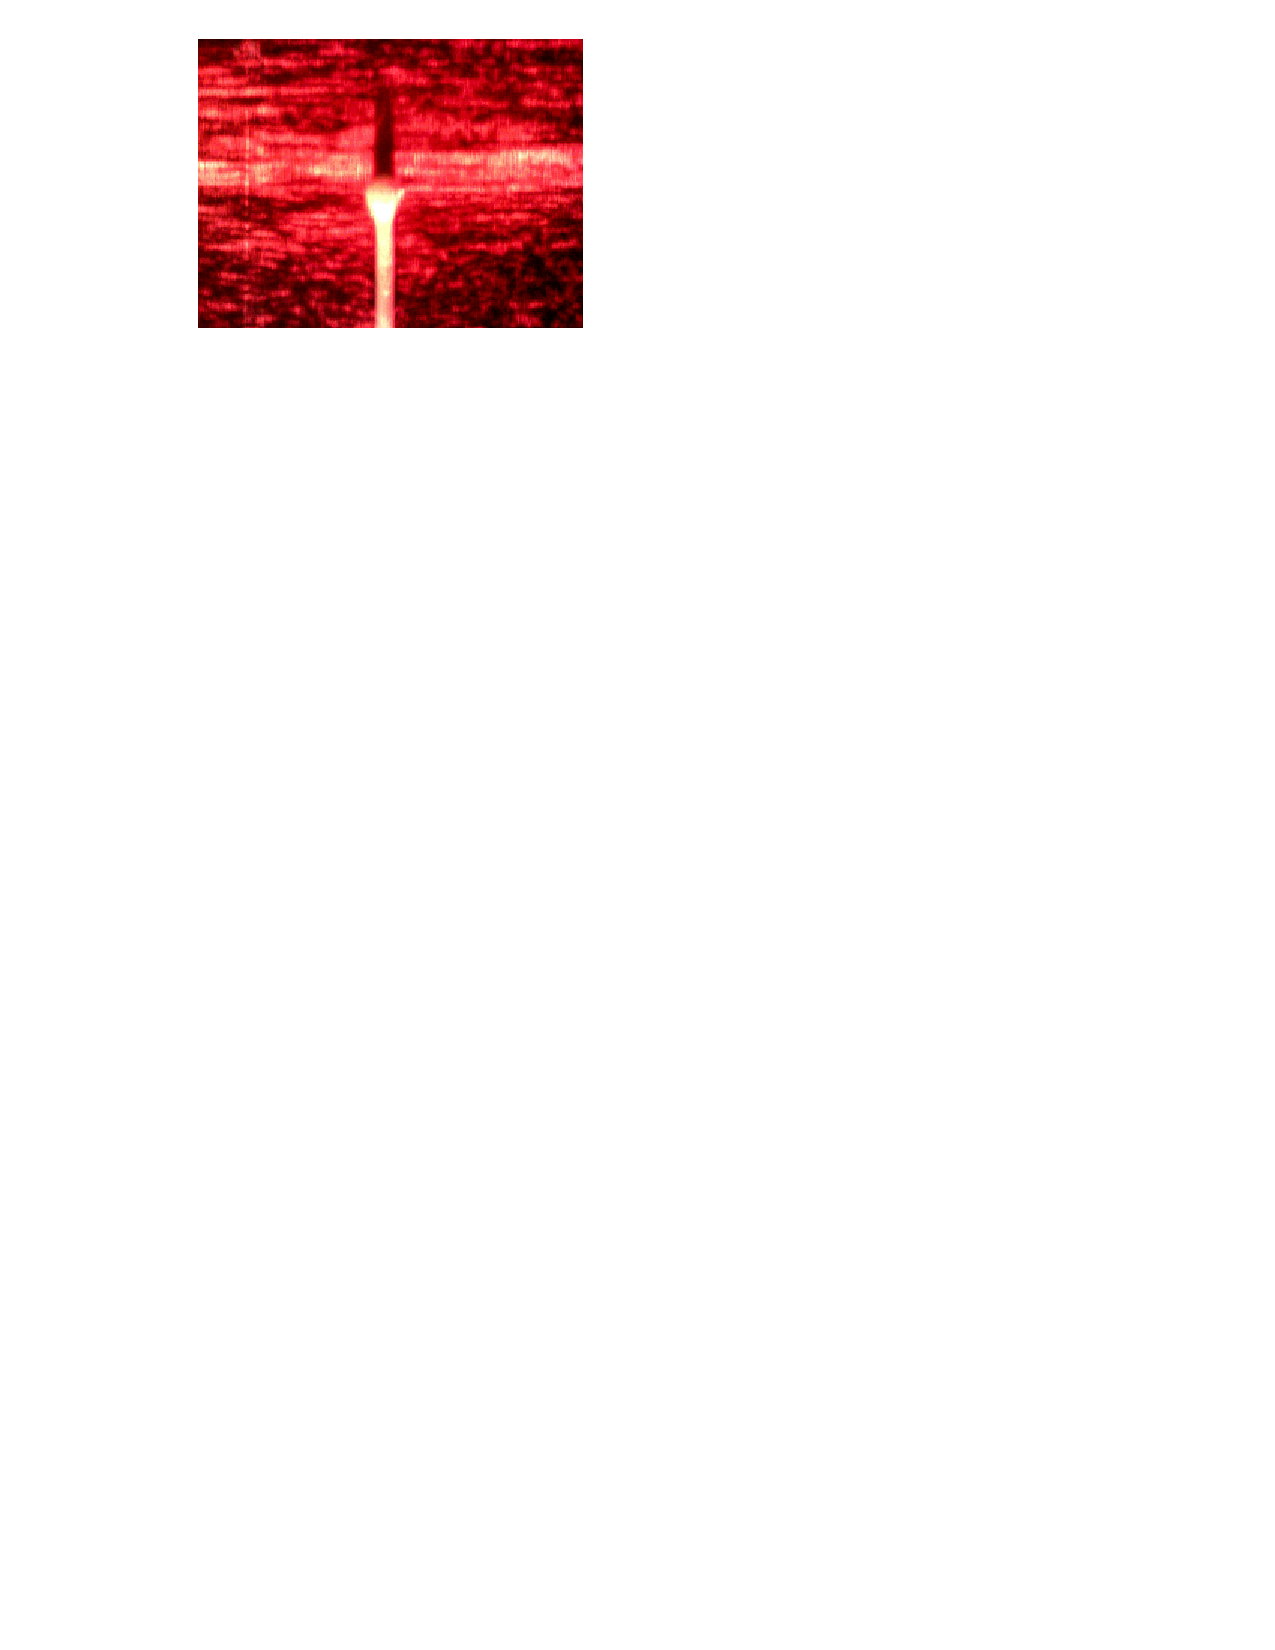
\includegraphics[width=1\textwidth]{data.pdf} 
	\setlength{\unitlength}{0.1\textwidth}
   	\footnotesize\put(-2,2.5){Laser line on bed}
   	\footnotesize\put(-2,2){Laser line on}
	\footnotesize\put(-2,1.7){deposition with}
	\footnotesize\put(-2,1.4){saturation}
	\footnotesize\put(-2,3.5){Reflections due to}
	\footnotesize\put(-2,3.2){Lens distortion}
   	\footnotesize\put(-9,3.5){Inclusion}
   	\footnotesize\put(-9.5,1.8){Inhomogeneous}
	\footnotesize\put(-9.5,1.5){Laser Line}
	\thicklines
	\color{brown}\put(-2.2,3.5){\vector(-1,0){2.5}}
	\color{brown}\put(-2.2,2.55){\vector(-1,0){1}}
	\color{brown}\put(-2.2,2){\vector(-1,0){2.9}}
	\color{brown}\put(-8,3.5){\vector(4,-1){2.9}}
	\color{brown}\put(-8,1.7){\vector(3,1){2}}
	\caption{Image from vision system with applicable terms to image sections.}
	\label{fig: data_problem}
\end{figure}

\skippar
% explain the lens distortion/ inhomogenity / impurities
Around the laser line are scattered reflections visible. A perfect laser should focus all light to a single line. The laser module is thought to be the source of this artifact. The lens in front of the laser beam converts the shape from a dot to a line. If there are any distortions/inhomogenities in or impurities on the lens this could result in a scattered line laser beam. Figure \ref{fig: data_problem} shows \textbf{inhomogenity in the laser line and reflections of light at unwanted places.} Since the laser will be operating in environmenst with heat an plastic materials it is possible that the lens gets contaminated. 

% explain hard to identify difference between distortion/impurty reflection vs real reflection on deposition
Reflections onto the print bed which do not belong to the real laser line have made it harder for the algorithm to detect where their seperation lays. Identifying whether the reflections on the deposition are generated by the unwanted reflections or by the real laser line is much harder.  The bed is a relatively flat surface and the angle of incidence of the light is considered to be about the same across the bed. The deposition is not a flat surface and the angle of incidence differs. As a result \textbf{light reflected from the depostion is hard to  seperate in laser line and light due to lens impurities or distortion.} Furthermore, the \textbf{width of the laser line onto the bed can differ from the laser line onto the deposition.} A steep angle for example in the deposition might condence the laser line beam such that it appears smaller on the image.

% explain saturation
Next to the reflections there is \textbf{saturation of pixels} visible in the image. This problem might be solvable with different hardware for this kind of material with its reflective properties. Another material might however reflect less and pixels would not illuminated enough by the new hardware. Changing hardware according to the use of different materials is not realistic and the problem should therefore be handled in the detection algorithm.

\section{Previous Work} \label{sc: previous_work}
To design a new algorithm a literature review is done on image processing for laser triangulation based structured light applications. The process towards extraction of features to be measured differs and many image processing algorithm exist. The general approach for laser triangulation based images can be divided into three stages, image segmentation, line extraction and feature extraction as described in \cite{li2007recent}. This literature review summerizes the methods used and points out potential problems of certain methods when applied to the data as shown in Figure \ref{fig: data_problem}.

\subsection*{Image Segmentation}
The goal of segmentation is to divide the image into seperate parts. To improve computational efficiency it is common to reduce the image to the range-of-interest. Thresholding the image based on gray-scale intensity is often used to seperate the structured light from the image background. To reduce disturbances in the image filters are usually applied before the thresholding.

\paragraph{Range-of-Interest}
A common first step is to reduce the size of the image to the so called range-of-interest (ROI) to reduce computation time. Manual selection of region size and position as in \cite{huang2012development} is only effective for detection of static positioned objects. Another paper \cite{wang2014weld} manually selects the column and/or row size of the ROI while row or column position is determined by the peak of the average column intensity of the image in gray-scale. This allows the object to move around while region size should be approximately constant. An algorithm to find the ROI position in both directions and determine the size automatically is described in \cite{xu2004features} where a manual threshold is set to seperate back and fore ground. The bounding box is determined by the maximum and minimum positions of the pixels left after thresholding. 

\skippar
Potential Problems:
\begin{itemize}
\item \textit{Information Loss} \label{pblm: info_loss} \\
Reducing the image size ignores potential information left in the sections outside of the ROI. The laser line outside of the region holds information on the laser line position and size for example. \textbf{Since inhomogenity of the laser line and disturbed areas are a problem as discussed in Section \ref{sc: data limitations} it is not recommended to conduct all further analyses based upon a ROI to prevent important information loss.}
\item \textit{Flexibility} \label{pblm: flexibility} \\
Gray-scale single channel images are used for determination of the ROI based upon the pixel intensity. Since most images are colored and consist out of three channels a lot of information is lost. As long as images are used where the structured light is clearly seperable from the background by gray-scale intensity this is not a problem. Our case however shows a difference in laser reflection on the bed and on the deposition. Usage of different materials might result in different reflections. \textbf{To prepare for different deposition materials it is not recommended to choose a ROI based upon gray-scale intensity since the light reflected from the deposition might not only differ in intensity.} 
\end{itemize}

\paragraph{Noise canceling} \label{p: noise_canceling}
The distinction between the laser line and background regions is often disturbed by noise. Convolution based filtering with different kernel size and shapes are often used. Paper \cite{huang2012development} uses a Gaussian shaped kernel of size $7x7$ to smooth the image. In \cite{zhang2007vision} a median filter is used where each pixel value is replaced by the median of neigbouring pixels. There are also frequency based filtering methods as applied in \cite{uzun2005fpga} and wavelet methods as in \cite{liu2006image}. Next to filtering in the spatial domain there are also papers which filter in the time domain. Removing noise by taking the smallest intensity of each pixel from consequtive images is described in \cite{li2010measurement}.

\skippar
Potential Problems:
\begin{itemize}
\item \textit{Information Loss} \label{pblm: info_loss2} \\
Smoothing the image by filtering removes noise and might remove important information on the exact point of seperation between the background and the structured light. 
\item \textit{Parameter Tuning} \label{pblm: parameter_tuning} \\
Every filter technique requires a choice for either a kernel size, cutoff-frequency or lag window. It is possible to automate the process at the cost of added complexity. 
\item \textit{Past Data Influence} \label{pblm: past_data} \\
Noise removal by averaging the data over consquetive images will smooth out the algorihms measurements over time. \textbf{The problems above give reason to avoid filters where possible.}
\end{itemize}

\paragraph{Laser segmentation}
For separation between laser line and background thresholding methods based upon gray-scale pixel value are commonly used. One of the simplest methods is described in \cite{zhang2007vision} where a fixed threshold value is determined by inspection of the image histogram. In \cite{wang2014weld} the threshold value is automatically determined by using the average of the maximum an minimum pixel intensity. A commonly used histogram thresholding method based upon maximizing the variance between the back and foreground is Otsu's method \cite{otsu1979threshold}. Also entropy based methods exist such as in \cite{liu2006image}. Next to the global thresholding methods described above there also exist local adaptive methods which adjust threshold locally. An image processing library which implements the most used methods for thresholding is described in \cite{itseez2015opencv}.

\skippar
Potential Problem:
\begin{itemize}
\item \textit{Position Independence} \label{pblm: pos_ind} \\
The threshold value of the local and global methods are only determined by either its neigbouring pixels or all pixels. The purpose of thresholding is to seperate background and foreground at the point of seperation. \textbf{Pixels far from the point of seperation between segments are not important. The methods used by the literature do not utilize this property.}
\end{itemize}

\subsection*{Laser Line Extraction} \label{ssc: line extraction}
The goal of line extraction is to convert the segment holding the laser light to a vector of pixel positions representing the laser line. 

\paragraph{Line Position}
% Back and Foreground segmentation
The most used method   \cite{nguyen2014laser} \cite{kim1995robust} \cite{li2010measurement} \cite{huang2012development} is to set the peak value of the gray-scale intensity of each column or row as the laser line position. Others \cite{davis2011vision} \cite{xu2004features} \cite{zhang2007vision} take the gradient of the segment edges and set the middle as the laser position. There also exist methods based upon morphology and the watershed algorithm as described in \cite{li2007recent}.

\skippar
Potential Problem:
\begin{itemize}
\item \textit{Gradients} \label{pblm: gradients} \\
Gradients are used to determine change. An advantage of this operation is computational efficiency while the disadvantage is that it is senstive to noise. Taking the derivative of a signal corrupted by noise will magnify the error. \textbf{Often peaks are determined from the gradient which is prone to errors if the Signal-To-Noise ratio is very low.}
\end{itemize}

\paragraph{Line Cleaning}
Noise makes it often impossible to detect the laser position for a column or row accurately. To account for these inhomogenities in the laser line interpolation in combination with an moving average filter can be used as described in \cite{wang2014weld}.

\subsection*{Feature Extraction}
After line extraction features to be measured are identified. Every application has its own features to detect. A common approach is to label certain point on the laser line as feature points. Dimensions can then be calculated by the difference between those points. The simplest methods \cite{li2010measurement} \cite{huang2012development} rely on taking second derivatives of the laser line and labeling the absolute values as feature points. In \cite{kim1995robust} the laser line is segmented into small sections connected t eachother (feature points) using polygonal fitting. Paper \cite{davis2011vision} decides if a point is a feature point based upon lingustic rules set by a threshold. 

